%% zusammenf.tex
%% $Id: zusammenf.tex 4 2005-10-10 20:51:21Z bless $
%%

\chapter{Diskussion \& Ausblick}
\label{ch:FutureWork}
%% ==============================
%

Wie in der Evaluation zu sehen ist, wurde die perfekte Lösung, eine Schlafapnoe mittels der eSense-Earpods zu ermitteln, noch nicht gefunden.
Es gibt Bereiche, in denen gute Resultate erzielt wurden, jedoch auch Bereiche, in denen Verbesserungspotenzial steckt. 

Ein Problem liegt möglicherweise darin, ab welcher Grenze ein Fenster als positiv markiert gilt.
Es wurde ein Fenster als positiv markiert deklariert, falls mehr als 50\% der Werte in diesem Fenster positiv markiert sind.
Somit wurde das Modell auch auf Fenster trainiert, welche knapp über 50\% positiv markierte Daten beinhalten.
Das betrifft die Regionen eines Übergangs zu einem Apnoeereignis oder von einem solchen weg.
Eine Lösung wäre, diese Fenster, welche den Übergang in ein Apnoeereignis beinhalten, zu verwerfen, wenn ein Modell trainiert wird. 
Das wurde in dieser Bachelorarbeit nicht getan, da dies auch bedeutet, dass die Anzahl der positiv markierten Fenster, worauf das Modell trainiert wird, kleiner wird.

Der Ausblick wird in zwei Bereiche aufgeteilt.
Der erste Bereich befasst sich mit den Signalen, welche zusätzlich in die Analyse mit aufgenommen werden können.
Im zweiten Bereich wird die Datenanalyse und die Klassifikation genauer betrachtet.

Zum ersten Bereich zählt das Mikrofonsignal, welches bei der Nutzerstudie zwar aufgezeichnet und persistiert wurde, jedoch in der Auswertung nicht mit eingeflossen ist. 
Das Mikrofonsignal kann weitere Informationen zur Detektion einer Schlafapnoe liefern. 
Mittels des Tonsignals direkt am Ohr können unter anderem die Atmung und auch der Puls herausgefiltert werden \cite{nomaWearableDataAcquisition2005}.
Diese Informationen können in die Auswertung mit einfließen und somit können die Erkenntnisse aus den IMU-Daten mit den Erkenntnissen des Mikrofonsignals zusammengeführt werden.

Im zweiten Bereich des Ausblicks wird erläutert, wie die Auswertung der zur Verfügung stehenden Daten verbessert werden kann.
Ein großer Nachteil der aktuellen Klassifikation eines Schlafapnoeereignisses ist, dass die Fenster nicht abhängig voneinander betrachtet werden.
Bei der aktuellen Klassifikation wird jedes Fenster separat und unabhängig von den anderen Fenstern klassifiziert.
Ein LSTM (\textit{Long short-term Memory}) würde hier die vorherigen bzw. nachfolgenden Fenster ebenfalls in Betracht ziehen und deren Entscheidung mit in die aktuelle Entscheidungsfindung einfließen lassen. 
Somit wird die Fehlerquote verringert, da potenzielle Outlier vermieden werden.

Zudem gibt es die Möglichkeit, die weiteren Features der IMU-Daten zu berechnen.
In dieser Bachelorarbeit wurden alle Features aus \texttt{tsfresh} mit in Betracht gezogen. 
Es könnten weitere Features in die Auswertung mit einfließen.
Es ist möglich, anhand der IMU-Daten das Puls- und $SPO_2$-Signal zu extrahieren. 
Diese beiden Signale können dann als Feature pro Fenster weitere Erkenntnisse liefern.
In der Abbildung \ref{futureWork:pulseSpo2} ist eine Beispielmessung eines Probanden zu sehen. 
In blau sind die Phasen zu sehen, in denen der Proband die Luft angehalten hat.
Hier ist der Wert auf 1 gesetzt, wenn die Person die Luft angehalten hat, ansonsten ist der Wert auf 0. 
In grün ist das $SpO_2$-Signal zu sehen, in orange das Pulssignal. 
Das $SpO_2$-Signal zeigt einen Abstieg nach dem Luftanhalten, ebenso steigt der Puls nach dem Luftanhalten.
Wenn dieses Signal mit in die Features mit aufgenommen wird, könnte ebenfalls die Genauigkeit der Klassifikation steigen. 
\begin{figure}[ht]
    \centering
    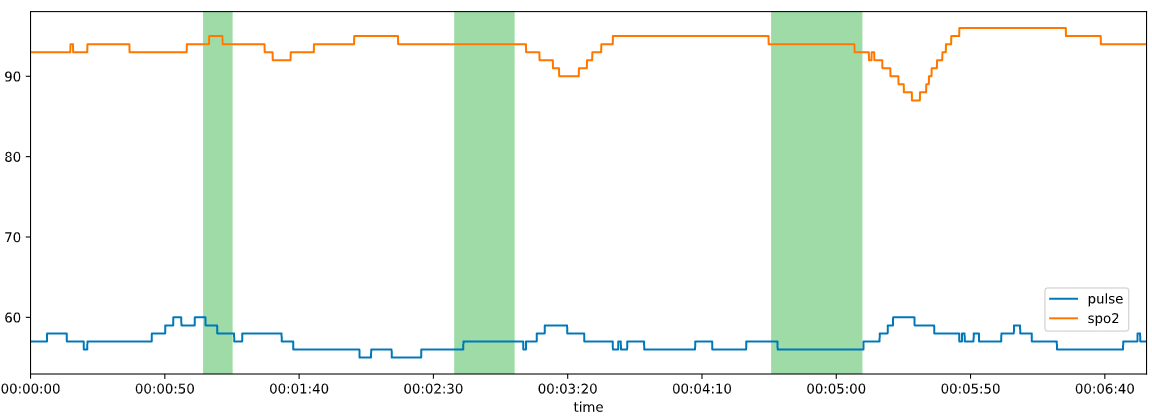
\includegraphics[width=1\textwidth]{futureWork/pulseSpo2_edited}
    \caption{Darstellung des Pulses und $SpO_2$-Signals einer Messung an einem Probanden. Beide Signale wurden aus den IMU-Daten der eSense-Earpods herausgefiltert. Das $SpO_2$-Signal zeigt Einbrüche an genau den 3 Stellen, an denen der Proband die Luft angehalten hat. Der Puls ist in diesen Bereichen ebenfalls minimal gestiegen. In grün sind die Bereiche markiert, in denen der Proband die Luft angehalten hat.}
    \label{futureWork:pulseSpo2}
\end{figure}

Eine weitere Möglichkeit bietet sich, indem die Zusatzinformationen der Nutzer mit in die Klassifikation eingebunden werden.
Hier können Personen des gleichen Geschlechts, Gewichts oder des gleichen Schlafrhythmusses in einem Modell trainiert werden.
Dies könnte mögliche Einflussfaktoren eliminieren und das Ergebnis ebenfalls verbessern.

Ein weiterer Ansatz zur Weiterarbeit an diesem Thema wird in \cite{perslevUTimeFullyConvolutional2019} behandelt.
Dort wird der Ansatz, Convolutional Layer und Recurrent Layer zu kombinieren und daraus sinnvolle Features zu extrahieren, betrachtet. 
Zudem werden zeitliche Beziehungen gefunden, was jedoch schwer zu ermitteln ist. 
Das Paper veröffentlicht \textit{U-Time}, einen zeichlichen, vollständigen Deep Learning Ansatz zur Analyse von physiologischen Zeitreihensegmenten. 
\textit{U-Time} wurde explizit zur Analyse von Schlafdaten entwickelt.
Jeder Zeitpunkt des Eingangssignals wird implizit klassifiziert, anschließend wird durch Aggregation dieser Klassifikation über feste Intervalle eine endgültige Vorhersage gebildet.